\subsection{Text recognition}
\label{sec:textrec}

This subsection describes the neural network that decodes a handwritten line image into text (functional unit FU~2.3 of the proposal, requirement R2).
The network, its training procedure and the layer library that trains it and runs it on the single-board computer were designed and written by the student.
No machine-learning library is used in the recogniser, the writer classifiers of Section~\ref{sec:writerid} or the forced alignment of Section~\ref{sec:styleprofile}: forward passes, backward (gradient) passes and optimiser updates are all evaluated by the student's own code (Section~\ref{sec:textrec-numpynn}).

\subsubsection{Problem statement and design approach}

The input is one grey-scale image of a text line from the segmentation block (Section~\ref{sec:segmentation}); the output is the string that was written.
Three properties of handwriting determine the design.
First, cursive characters are joined, so their boundaries cannot be located reliably; cutting the line into characters and classifying each piece, as the proposal planned, would pass every cutting error into a wrong reading.
Second, the number of characters is unknown and has no fixed relation to image width, since the same letter can be written narrow or wide.
Third, the available training material (public handwriting databases and the personal pages of the two writers) gives line images with transcriptions, but not the position of every character.
The design that follows from these three properties is reviewed against its alternatives at the end of this subsection.

The design is therefore a \emph{convolutional neural network (CNN)} followed by a \emph{bidirectional long short-term memory (BiLSTM)} network and trained with \emph{connectionist temporal classification (CTC)}~\cite{graves2006,shi2017}: the convolutional layers turn the image into one feature vector per narrow vertical slice, the recurrent layers give every slice the context of the whole line, and the CTC loss allows training from the line transcription alone, with no alignment between characters and columns.
The layer pattern follows a published design for the IAM handwriting database~\cite{kizilirmak2023}; the student fixed the input geometry, built the data pipeline and the training recipe, and verified every layer shape and parameter count (Table~\ref{tab:rec-layers}).

\subsubsection{Input pre-processing}

The input size is fixed at $64\times640$ pixels, which allows batching and a fixed sequence length; it is smaller than the $100\times960$ of the published design, which needed about one hour per training epoch on a processor-only computer.
A line crop of height $h$ and width $w$ pixels is resized \emph{uniformly} (the aspect ratio is preserved) with the scale
\begin{equation}
s=\min\!\Bigl(\frac{64}{h},\frac{640}{w}\Bigr),\qquad w'=\max(1,\mathrm{round}(ws)),\qquad h'=\max(1,\mathrm{round}(hs)),
\label{eq:rec-resize}
\end{equation}
using bilinear interpolation (Equation~\ref{eq:seg-resize}), and pasted onto a white $640\times64$ canvas, left-aligned and vertically centred (Figure~\ref{fig:rec-canvas}), the left alignment making the conversion from a network time step back to a pixel position in the original crop an exact inverse, $x_{\mathrm{orig}}=x_{\mathrm{canvas}}/s$, which the style-extraction block (Section~\ref{sec:styleprofile}) needs when it cuts characters out of lines.
Typical text lines are about $14{:}1$ in width to height and the canvas is $10{:}1$, so for most lines the width binds in Equation~\ref{eq:rec-resize} and the line occupies fewer than 64 rows.
A plain stretch to the canvas was used initially but distorted letter proportions: in one example it applied a horizontal scale of 0.48 against a vertical scale of 0.35, which is why the uniform scale of Equation~\ref{eq:rec-resize} replaced it.
The grey values $p\in[0,255]$ are then inverted and normalised by Equation~\ref{eq:rec-norm},
\begin{equation}
x=\frac{(1-p/255)-0.5}{0.5}=1-\frac{2p}{255},
\label{eq:rec-norm}
\end{equation}
where $x\in[-1,1]$ is the network input: white paper ($p=255$) becomes $-1$ and black ink ($p=0$) becomes $+1$ in Equation~\ref{eq:rec-norm}.
The constant of Equation~\ref{eq:rec-norm} is \emph{fixed} rather than a per-image mean and standard deviation, so the amount of white padding cannot change the contrast statistics.
Figure~\ref{fig:rec-canvas} shows the complete pre-processing geometry.

\begin{figure}[h]
\centering
\begin{tikzpicture}[x=1cm,y=1cm]
\draw[thick,fill=gray!15] (0,2.2) rectangle (5.6,3.3);
\node[font=\small] at (2.8,2.75) {line crop: $w\times h$ pixels, variable};
\draw[w2arr] (2.8,2.1) -- (2.8,1.4) node[midway,right,font=\small] {scale by $s$, Equation~\ref{eq:rec-resize}};
\draw[thick] (0,0) rectangle (8,0.8);
\draw[thick,fill=gray!15] (0,0.1) rectangle (5.6,0.7);
\node[font=\small] at (2.8,0.4) {scaled line $w'\times h'$};
\node[font=\small] at (6.8,0.4) {white padding};
\node[font=\small,anchor=east] at (-0.1,0.4) {64};
\node[font=\small,anchor=north] at (4,-0.05) {640 pixels};
\draw[<->] (-0.05,0) -- (-0.05,0.8);
\node[font=\small,align=left,anchor=west] at (8.5,0.4) {ink $\rightarrow+1$\\ paper $\rightarrow-1$};
\end{tikzpicture}
\caption{Pre-processing of a line crop. The crop is scaled uniformly, left-aligned on a white canvas and normalised to the range $[-1,1]$ (Equation~\ref{eq:rec-norm}).}
\label{fig:rec-canvas}
\end{figure}


\subsubsection{Network architecture}

The $1\times64\times640$ input passes through three convolutional stages of 32, 64 and 128 channels separated by two $2\times2$ max-pools, which leaves a $128\times16\times160$ feature map; a maximum over the height turns it into 160 vectors, two bidirectional LSTM layers of hidden size 256 per direction give $160\times512$, and a linear layer with log-softmax gives the $160\times75$ scores that greedy CTC decoding turns into text.
Figure~\ref{fig:rec-arch} is the overview diagram of those stages with their tensor shapes, and Table~\ref{tab:rec-layers} lists every layer with its shape and parameter count; the building blocks are defined first.

\begin{figure}[h]
\centering
\begin{tikzpicture}[x=1cm,y=1cm]
\tikzset{nb/.style={w2box,text width=2.55cm,minimum height=1.5cm}}
\node[nb] (in) at (-6.2,0) {\textbf{Input}\\ $1\times64\times640$};
\node[nb] (s1) at (-3.1,0) {\textbf{Stage 1}\\ 2$\times$[conv 3$\times$3, BN, ReLU], 32 ch.\\ $32\times64\times640$};
\node[nb] (p1) at (0,0) {\textbf{Max-pool 2$\times$2}\\ $32\times32\times320$};
\node[nb] (s2) at (3.1,0) {\textbf{Stage 2}\\ 4$\times$[conv, BN, ReLU], 64 ch.\\ $64\times32\times320$};
\node[nb] (p2) at (6.2,0) {\textbf{Max-pool 2$\times$2}\\ $64\times16\times160$};
\node[nb] (s3) at (6.2,-2.3) {\textbf{Stage 3}\\ 6$\times$[conv, BN, ReLU], 128 ch.\\ $128\times16\times160$};
\node[nb] (hm) at (3.1,-2.3) {\textbf{Height max-pool}\\ $128\times1\times160$\\ $\rightarrow$ 160 vectors};
\node[nb] (ls) at (0,-2.3) {\textbf{BiLSTM $\times2$}\\ hidden 256 per direction\\ $160\times512$};
\node[nb] (ln) at (-3.1,-2.3) {\textbf{Linear + log-softmax}\\ $160\times75$};
\node[nb] (dc) at (-6.2,-2.3) {\textbf{Greedy CTC decoding}\\ collapse repeats, delete blanks $\rightarrow$ text};
\foreach \a/\b in {in/s1,s1/p1,p1/s2,s2/p2,p2/s3,s3/hm,hm/ls,ls/ln,ln/dc} \draw[w2arr] (\a)--(\b);
\end{tikzpicture}
\caption{Architecture of the text recogniser. Tensor shapes are channels $\times$ height $\times$ width for the convolutional part and time steps $\times$ features for the recurrent part; BN denotes batch normalisation.}
\label{fig:rec-arch}
\end{figure}

\begin{table}[h]
\centering
\fontsize{9.5}{11.5}\selectfont
\begin{tabular}{|l|l|r|}
\hline
\textbf{Layer} & \textbf{Output shape} & \textbf{Trainable parameters} \\
\hline
Input & $1\times64\times640$ & 0 \\
Conv 3$\times$3 (1$\to$32), BN, ReLU & $32\times64\times640$ & 384 \\
Conv 3$\times$3 (32$\to$32), BN, ReLU & $32\times64\times640$ & 9\,312 \\
Max-pool 2$\times$2 & $32\times32\times320$ & 0 \\
Conv 3$\times$3 (32$\to$64), BN, ReLU & $64\times32\times320$ & 18\,624 \\
3$\times$ Conv 3$\times$3 (64$\to$64), BN, ReLU & $64\times32\times320$ & 111\,168 \\
Max-pool 2$\times$2 & $64\times16\times160$ & 0 \\
Conv 3$\times$3 (64$\to$128), BN, ReLU & $128\times16\times160$ & 74\,112 \\
5$\times$ Conv 3$\times$3 (128$\to$128), BN, ReLU & $128\times16\times160$ & 739\,200 \\
Height max-pool & $128\times1\times160$ & 0 \\
BiLSTM layer 1 (128$\to$256, 2 directions) & $160\times512$ & 790\,528 \\
BiLSTM layer 2 (512$\to$256, 2 directions) & $160\times512$ & 1\,576\,960 \\
Linear (512$\to$75) & $160\times75$ & 38\,475 \\
Log-softmax & $160\times75$ & 0 \\
\hline
\textbf{Total} & & \textbf{3\,358\,763} \\
\hline
\end{tabular}
\caption{Layer-by-layer shapes and trainable parameters of the text recogniser (batch dimension omitted). Batch normalisation also stores 2\,176 non-trainable running statistics, so the from-scratch checkpoint \texttt{paper\_cnn\_bilstm\_ctc\_scratch\_best.npz} holds $3\,358\,763+2\,176=3\,360\,939$ numbers in 90 arrays (13.4\,MB as 32-bit floating point). The earlier checkpoints converted from the framework runs hold the same 3\,360\,939 weights and statistics in 102 arrays, 3\,360\,951 numbers in all, the twelve extra entries being per-layer batch counters that play no part in the forward pass and are not used anywhere in this report.}
\label{tab:rec-layers}
\end{table}

\paragraph{Two-dimensional convolution.}
A convolutional layer slides a small learned filter over the image, so the same pattern detector (for example a stroke end or a loop) acts at every position.
For an input feature map $X$ with $C_{\mathrm{in}}$ channels, the output channel $o$ at position $(i,j)$ is Equation~\ref{eq:rec-conv},
\begin{equation}
Y[o,i,j]=b_o+\sum_{c=1}^{C_{\mathrm{in}}}\sum_{u=0}^{k-1}\sum_{v=0}^{k-1}W[o,c,u,v]\;X_{\mathrm{pad}}[c,\,s\,i+u,\,s\,j+v],
\label{eq:rec-conv}
\end{equation}
with $W$ the learned weights, $b_o$ the bias of channel $o$, $k$ the kernel size, $s$ the stride and $X_{\mathrm{pad}}$ the input zero-padded by $p$ pixels on every side.
The output size follows from the same kernel size, padding and stride by Equation~\ref{eq:rec-outsize},
\begin{equation}
H_{\mathrm{out}}=\Bigl\lfloor\frac{H+2p-k}{s}\Bigr\rfloor+1,\qquad W_{\mathrm{out}}=\Bigl\lfloor\frac{W+2p-k}{s}\Bigr\rfloor+1,
\label{eq:rec-outsize}
\end{equation}
where $H$ and $W$ are the input height and width and $H_{\mathrm{out}}$, $W_{\mathrm{out}}$ those of the output; Equation~\ref{eq:rec-outsize} is what fixes every tensor shape of Table~\ref{tab:rec-layers}.
For the values used here, $k=3$, $p=1$ and $s=1$, Equation~\ref{eq:rec-outsize} returns the input size, so only pooling changes the size, and a layer has $C_{\mathrm{out}}(C_{\mathrm{in}}k^2+1)$ parameters.
Equation~\ref{eq:rec-conv} is the expression from which the forward and the backward pass of the layer were derived by hand (Section~\ref{sec:textrec-numpynn}), and its six nested summations are also the reason the implementation does not evaluate it directly.
Instead the padded input of each convolution is cut into overlapping $k\times k$ patches that become the columns of a matrix $\mathrm{cols}$, and the whole layer is evaluated as the single matrix product of Equation~\ref{eq:rec-im2col} (the im2col method~\cite{chellapilla2006}),
\begin{equation}
Y=\tilde W\,\mathrm{cols}+b\,\mathbf 1^{\top},
\label{eq:rec-im2col}
\end{equation}
where $\tilde W\in\mathbb R^{C_{\mathrm{out}}\times C_{\mathrm{in}}k^2}$ is the weight tensor of Equation~\ref{eq:rec-conv} reshaped to a matrix, $\mathrm{cols}\in\mathbb R^{(C_{\mathrm{in}}k^2)\times(H_{\mathrm{out}}W_{\mathrm{out}})}$ holds one flattened $3\times3$ patch per column, and $b\,\mathbf 1^\top$ adds the channel bias at all positions.
Equation~\ref{eq:rec-im2col} is the same sum as Equation~\ref{eq:rec-conv} rearranged, so it changes the cost and not the result: one optimised matrix product replaces the six nested loops of Equation~\ref{eq:rec-conv} and was found to be about ten times faster than a general summation routine, with a difference of about $10^{-13}$ between the two.
The cost is memory. The largest matrix, for the second convolution of stage 1, has $288\times40\,960$ entries (47\,MB as 32-bit floating point), and the largest activation tensor is 5.2\,MB, so the working set of Equation~\ref{eq:rec-im2col} is a few tens of megabytes.

\paragraph{Batch normalisation, rectified linear unit and pooling.}
Deep networks train poorly if the distribution of each layer's inputs keeps changing, so every convolution is followed by batch normalisation~\cite{ioffe2015} and the rectified linear unit $\mathrm{ReLU}(x)=\max(0,x)$~\cite{nair2010}, and a $2\times2$ max-pooling with stride 2~\cite{lecun1998} halves height and width, tolerates small shifts and has no parameters.
During training, for each channel the mean $\mu_B$ and variance $\sigma_B^2$ are computed over the mini-batch and all spatial positions, and the output is Equation~\ref{eq:rec-bn},
\begin{equation}
\hat x=\frac{x-\mu_B}{\sqrt{\sigma_B^2+\varepsilon}},\qquad y=\gamma\hat x+\beta,\qquad\varepsilon=10^{-5},
\label{eq:rec-bn}
\end{equation}
where $\gamma$ and $\beta$ are the learned scale and shift parameters of the channel in Equation~\ref{eq:rec-bn}.
Running averages of the mean and variance are kept during training, and at test time they replace $\mu_B$ and $\sigma_B^2$, which turns the layer into the fixed per-channel affine map $y=a\,x+b$ of Equation~\ref{eq:rec-bnfold},
\begin{equation}
a=\frac{\gamma}{\sqrt{\sigma^2_{\mathrm{run}}+\varepsilon}},\qquad b=\beta-a\,\mu_{\mathrm{run}},
\label{eq:rec-bnfold}
\end{equation}
where $\mu_{\mathrm{run}}$ and $\sigma^2_{\mathrm{run}}$ are the running statistics; the folded form of Equation~\ref{eq:rec-bnfold} is exactly the form that the inference implementation uses.
The $2\times2$ max-pooling outputs the maximum of each block, $Y[c,i,j]=\max_{u,v\in\{0,1\}}X[c,2i+u,2j+v]$, where $X$ is the input feature map, $Y$ the output, $c$ the channel and $(i,j)$ the output position.
After the last convolution the remaining 16 rows are collapsed by a maximum over the height, Equation~\ref{eq:rec-hmax},
\begin{equation}
z_t[c]=\max_{i}F[c,i,t],\qquad t=1,\ldots,T=160,
\label{eq:rec-hmax}
\end{equation}
where, in Equation~\ref{eq:rec-hmax}, $F$ is the output of the last convolutional stage, $c$ the channel, $i$ the row and $z_t\in\mathbb R^{128}$ the feature vector of step $t$; the height collapse is therefore a maximum over a whole column rather than over a $2\times2$ block.
The collapse of Equation~\ref{eq:rec-hmax} discards the vertical position and keeps only whether a feature is present anywhere in the column, which suits the ascenders and descenders of handwriting, and it turns the two-dimensional map into a one-dimensional sequence; the two pools halve the width twice, so $T=640/4=160$ steps remain and one step covers a four-pixel-wide column group.
The region of the input that influences one feature is found with the recursion of Equation~\ref{eq:rec-rf}, in which $r$ is the receptive field and $j$ the distance in input pixels between adjacent features (the jump).
\begin{equation}
r_{\mathrm{out}}=r_{\mathrm{in}}+(k-1)\,j_{\mathrm{in}},\qquad j_{\mathrm{out}}=j_{\mathrm{in}}\,s.
\label{eq:rec-rf}
\end{equation}
Applied to the network (two convolutions, a pool, four convolutions, a pool, six convolutions) Equation~\ref{eq:rec-rf} gives 5, 6, 22, 24 and finally 72 pixels, so each column feature has a receptive field of $72\times72$ pixels, the full height of the line and about 18 time steps of context, before the recurrent layers add unbounded horizontal context.

\paragraph{Long short-term memory.}
The recurrent part reads the 160 feature vectors in order. A plain recurrent network forgets information over long sequences, so a long short-term memory (LSTM) cell~\cite{hochreiter1997} is used, whose memory is protected by a forget, an input and an output gate (Figure~\ref{fig:rec-lstm}).
For input $x_t$ and the previous hidden state $h_{t-1}$ and memory $c_{t-1}$ (both initially zero), one direction of one layer with hidden size $n=256$ computes Equation~\ref{eq:rec-lstm},
\begin{equation}
\begin{aligned}
i_t&=\sigma(W_{ii}x_t+b_{ii}+W_{hi}h_{t-1}+b_{hi}), &&\text{input gate,}\\
f_t&=\sigma(W_{if}x_t+b_{if}+W_{hf}h_{t-1}+b_{hf}), &&\text{forget gate,}\\
g_t&=\tanh(W_{ig}x_t+b_{ig}+W_{hg}h_{t-1}+b_{hg}), &&\text{candidate memory,}\\
o_t&=\sigma(W_{io}x_t+b_{io}+W_{ho}h_{t-1}+b_{ho}), &&\text{output gate,}\\
c_t&=f_t\odot c_{t-1}+i_t\odot g_t,\qquad h_t=o_t\odot\tanh(c_t),
\end{aligned}
\label{eq:rec-lstm}
\end{equation}
with, in Equation~\ref{eq:rec-lstm}, $\sigma(a)=1/(1+e^{-a})$ the logistic function, $\odot$ the element-wise product, the $W$ weight matrices (input $W_{i\cdot}$, recurrent $W_{h\cdot}$) and the $b$ bias vectors.
The forget gate sets how much old memory is kept, the input gate how much of the candidate is written and the output gate how much is revealed.
In the implementation the four pre-activations of Equation~\ref{eq:rec-lstm} come from one product, $[i;f;g;o]=W_{ih}x_t+b_{ih}+W_{hh}h_{t-1}+b_{hh}$ with $W_{ih}\in\mathbb R^{1024\times I}$ and $W_{hh}\in\mathbb R^{1024\times256}$, the four blocks of rows being the four gates of Equation~\ref{eq:rec-lstm}.
A \emph{bidirectional} layer~\cite{schuster1997} runs one LSTM from step 1 to 160 and an independent second from 160 to 1, and concatenates their hidden states at every step as in Equation~\ref{eq:rec-bi},
\begin{equation}
h_t=\bigl[\,\overrightarrow{h}_t\,;\,\overleftarrow{h}_t\,\bigr]\in\mathbb R^{512},
\label{eq:rec-bi}
\end{equation}
in which $\overrightarrow{h}_t$ and $\overleftarrow{h}_t$ are the 256-dimensional states of the forward and the backward direction at step $t$, so each step of Equation~\ref{eq:rec-bi} sees the letters before and after it, which is needed to distinguish the cursive strokes of u, n and m.
Two such bidirectional layers are stacked, with no dropout, following the published design.

\begin{figure}[h]
\centering
\begin{tikzpicture}[x=1cm,y=1cm]
\draw[thick,rounded corners=3pt] (0,0) rectangle (8,3.6);
\node[w2box,minimum width=1cm] (f) at (1.4,1.2) {$\sigma$};
\node[w2box,minimum width=1cm] (i) at (3.0,1.2) {$\sigma$};
\node[w2box,minimum width=1cm] (g) at (4.6,1.2) {$\tanh$};
\node[w2box,minimum width=1cm] (o) at (6.6,1.2) {$\sigma$};
\node[font=\scriptsize] at (1.4,0.55) {$f_t$};
\node[font=\scriptsize] at (3.0,0.55) {$i_t$};
\node[font=\scriptsize] at (4.6,0.55) {$g_t$};
\node[font=\scriptsize] at (6.6,0.55) {$o_t$};
\draw[thick,-{Stealth}] (-0.8,3.0) -- (8.8,3.0) node[right,font=\small] {$c_t$};
\node[font=\small,left] at (-0.8,3.0) {$c_{t-1}$};
\node[w2dark,circle,inner sep=1pt] (m1) at (1.4,3.0) {$\odot$};
\node[w2dark,circle,inner sep=1pt] (a1) at (3.8,3.0) {$+$};
\node[w2dark,circle,inner sep=1pt] (m2) at (3.8,2.1) {$\odot$};
\node[w2box,minimum width=0.9cm] (th) at (6.6,3.0) {$\tanh$};
\node[w2dark,circle,inner sep=1pt] (m3) at (6.6,2.1) {$\odot$};
\draw[w2arr] (f) -- (m1);
\draw[w2arr] (i) |- (m2); \draw[w2arr] (g) |- (m2); \draw[w2arr] (m2) -- (a1);
\draw[w2arr] (o) -- (m3); \draw[w2arr] (th) -- (m3);
\draw[w2arr] (m3) -- ++(0,-2.6) -- ++(0,0);
\node[font=\small,anchor=west] at (7.0,2.1) {$h_t$};
\node[font=\small,anchor=north] at (4.0,-0.2) {inputs of all four gates: $[x_t,\,h_{t-1}]$};
\end{tikzpicture}
\caption{Schematic of an LSTM cell (Equation~\ref{eq:rec-lstm}). The memory line $c_t$ at the top is changed only by the forget gate (multiplication) and the input gate (addition), which allows information to travel over many time steps.}
\label{fig:rec-lstm}
\end{figure}


\paragraph{Output layer and parameter count.}
A linear layer maps the 512-dimensional state of each step to one score $\ell_t^k$ for each of the 75 classes (74 characters and one blank, index 0), and a log-softmax turns the scores into the log-probabilities of Equation~\ref{eq:rec-softmax},
\begin{equation}
\ell_t=W_oh_t+b_o,\qquad \log y_t^k=\ell_t^k-\log\sum_{j=0}^{74}e^{\ell_t^j},
\label{eq:rec-softmax}
\end{equation}
with, in Equation~\ref{eq:rec-softmax}, $h_t\in\mathbb R^{512}$ the bidirectional state of step $t$, $W_o\in\mathbb R^{75\times512}$ and $b_o$ the learned weights and bias, and $y_t^k=P(\pi_t=k\mid x)$ the probability of class $k$ at step $t$.
The 74 symbols of Equation~\ref{eq:rec-softmax} are the 26 lower-case and 26 upper-case letters, the ten digits and twelve symbols (space and . , ; : ' " ! ? ( ) -).
Characters outside this set are removed from every label, lines that become empty are dropped, and lines of more than 120 characters, which indicate merged lines, are dropped.

The counts of Table~\ref{tab:rec-layers} follow from the layer shapes.
A convolution with batch normalisation has $C_{\mathrm{out}}(9C_{\mathrm{in}}+1)+2C_{\mathrm{out}}$ trainable parameters, and one LSTM direction has the count of Equation~\ref{eq:rec-params},
\begin{equation}
N_{\mathrm{LSTM}}=4n(I+n)+2\cdot4n,
\label{eq:rec-params}
\end{equation}
with $I$ the input size, $n=256$ the hidden size and the last term of Equation~\ref{eq:rec-params} the two bias vectors; the first layer gives $N=4\cdot256\cdot384+2048=395\,264$ and the second $788\,480$ per direction.
The network holds 3\,358\,763 parameters, of which the LSTM layers hold 70.5\,\%, stage 3 24.2\,\%, stage 2 3.9\,\%, the output layer 1.1\,\% and stage 1 0.3\,\%.
The number of multiply--accumulate operations (MACs) for one line is Equation~\ref{eq:rec-macs},
\begin{equation}
\begin{split}N_{\mathrm{MAC}}={}&\sum_\ell 9\,C_{\mathrm{in},\ell}C_{\mathrm{out},\ell}H_\ell W_\ell\\&+2T\,[4n(128+n)+4n(512+n)]+T\cdot512\cdot75\approx4.17\times10^9,\end{split}
\label{eq:rec-macs}
\end{equation}
with $H_\ell W_\ell$ the feature-map size at convolutional layer $\ell$ and $T=160$ the number of time steps: the three terms of Equation~\ref{eq:rec-macs} are $3.79\times10^9$ for the convolutions, $0.38\times10^9$ for the BiLSTM and $6\times10^6$ for the output layer.
Convolutions therefore dominate the arithmetic (91\,\%), while the LSTM is inherently sequential, with $160\times2\times2=640$ small matrix--vector products.

\subsubsection{Connectionist temporal classification}

The network outputs a distribution over 75 symbols at each of 160 steps, but the transcription has only, for example, 40 characters and its alignment with the steps is unknown; CTC solves this by summing over all alignments.
A \emph{path} $\pi=(\pi_1,\ldots,\pi_T)$ assigns one symbol, possibly the blank, to every step, and the many-to-one map $\mathcal B$ merges consecutive repeats and then deletes the blanks, so that $\mathcal B(\text{--hh-e-ll-ll-o})=\text{hello}$, the blank between the two groups of l allowing a genuine double letter.
With the steps conditionally independent, the probability of a transcription $y=(y_1,\ldots,y_U)$ of length $U$ is the sum over all paths that collapse to it, and the loss its negative logarithm:
\begin{equation}
P(\pi\mid x)=\prod_{t=1}^{T}y_t^{\pi_t},\qquad p(y\mid x)=\sum_{\pi:\,\mathcal B(\pi)=y}P(\pi\mid x),\qquad \mathcal L_{\mathrm{CTC}}=-\ln p(y\mid x).
\label{eq:rec-ctcprob}
\end{equation}
The number of paths is exponential in $T$, so the sum of Equation~\ref{eq:rec-ctcprob} is evaluated by the forward--backward dynamic programme of Graves \emph{et al.}~\cite{graves2006} on the blank-augmented label $y'=(\varnothing,y_1,\varnothing,y_2,\ldots,y_U,\varnothing)$ of length $S=2U+1$ (Figure~\ref{fig:rec-ctc}).
The forward variable $\alpha_t(s)$ is the total probability of all consistent path prefixes of length $t$ ending at position $s$ of $y'$, and obeys the recursion of Equation~\ref{eq:rec-alpha}:
\begin{equation}
\begin{split}&\alpha_1(1)=y_1^{\varnothing},\quad\alpha_1(2)=y_1^{y_1},\quad\alpha_1(s)=0\ (s>2),\\&\alpha_t(s)=\Bigl[\alpha_{t-1}(s)+\alpha_{t-1}(s-1)+\mathbb 1[\,y'_s\ne\varnothing\wedge y'_s\ne y'_{s-2}\,]\,\alpha_{t-1}(s-2)\Bigr]\,y_t^{\,y'_s},\end{split}
\label{eq:rec-alpha}
\end{equation}
where $y_t^{\varnothing}$ is the network's blank probability at step $t$, $y_t^{y'_s}$ the probability of the symbol at position $s$ of $y'$ and $\mathbb 1[\cdot]$ the indicator function.
The three bracket terms of Equation~\ref{eq:rec-alpha} are the allowed transitions into position $s$: staying on the same symbol, advancing one position, and skipping a blank to the next symbol.
The skip is forbidden when $y'_s$ is a blank or equals $y'_{s-2}$, since skipping the blank between two equal letters would merge them.
Carried to the last step, the recursion of Equation~\ref{eq:rec-alpha} gives the probability of the transcription as Equation~\ref{eq:rec-pfinal},
\begin{equation}
p(y\mid x)=\alpha_T(S)+\alpha_T(S-1),
\label{eq:rec-pfinal}
\end{equation}
where $T$ is the number of time steps and $S=2U+1$ the length of $y'$ for a transcription $y$ of $U$ characters.
The two terms of Equation~\ref{eq:rec-pfinal} are the paths that end on the last character of $y$ and those that end on the final blank of $y'$, which are the only two positions a complete alignment can occupy at step $T$, so the exponential sum of Equation~\ref{eq:rec-ctcprob} costs $O(TS)$ operations.
The backward variable $\beta_t(s)$ is the mirror image of $\alpha_t(s)$: it is the total probability of all consistent path \emph{suffixes} that start at position $s$ of $y'$ at step $t$ and reach the end of $y'$ at step $T$, and it obeys the recursion of Equation~\ref{eq:rec-beta}, run from $t=T$ downwards,
\begin{equation}
\begin{split}&\beta_T(S)=\beta_T(S-1)=1,\qquad\beta_T(s)=0\ (s<S-1),\\
&\beta_t(s)=\beta_{t+1}(s)\,y_{t+1}^{\,y'_s}+\beta_{t+1}(s+1)\,y_{t+1}^{\,y'_{s+1}}+\mathbb 1[\,y'_s\ne\varnothing\wedge y'_s\ne y'_{s+2}\,]\,\beta_{t+1}(s+2)\,y_{t+1}^{\,y'_{s+2}},\end{split}
\label{eq:rec-beta}
\end{equation}
where $S=2U+1$, $y_{t+1}^{\,y'_s}$ is the network's probability at step $t+1$ of the symbol standing at position $s$ of the blank-augmented label, terms with $s+1$ or $s+2$ beyond $S$ are zero, and $\mathbb 1[\cdot]$ forbids the same skip transition as Equation~\ref{eq:rec-alpha}.
The three terms of Equation~\ref{eq:rec-beta} are the reverses of the three transitions of Equation~\ref{eq:rec-alpha}, read forwards out of position $s$ instead of backwards into it, and the two non-zero initial values are the two positions a complete alignment may occupy at step $T$, the same two that Equation~\ref{eq:rec-pfinal} adds.
The emission at step $t$ itself is deliberately \emph{not} included in $\beta_t(s)$, which is why Equation~\ref{eq:rec-beta} multiplies by the probabilities of step $t+1$ and initialises $\beta_T$ to one rather than to $y_T^{\,y'_s}$; with that convention the product $\alpha_t(s)\beta_t(s)$ counts the emission $y_t^{\,y'_s}$ exactly once, since $\alpha_t(s)$ already carries it.
Equations~\ref{eq:rec-alpha} and~\ref{eq:rec-beta} together cost $O(TS)$ each and are the whole of the forward--backward dynamic programme.

From the two variables the gradient follows in closed form. The posterior probability that the alignment occupies position $s$ at step $t$, given the transcription, is the normalised product $\gamma_t(s)$ of Equation~\ref{eq:rec-ctcocc}; summing it over every position of $y'$ that carries class $k$ gives the \emph{occupancy} of that class at that step, and the gradient of the loss with respect to the pre-softmax score $\ell_t^k$ is the network's own probability less that occupancy,
\begin{equation}
\gamma_t(s)=\frac{\alpha_t(s)\,\beta_t(s)}{p(y\mid x)},\qquad \mathrm{occ}_t^{\,k}=\sum_{s:\,y'_s=k}\gamma_t(s),\qquad \frac{\partial\mathcal L}{\partial\ell_t^{k}}=y_t^k-\mathrm{occ}_t^{\,k},
\label{eq:rec-ctcocc}
\end{equation}
where $p(y\mid x)$ is the sequence probability of Equation~\ref{eq:rec-pfinal} and $y_t^k$ the softmax probability of class $k$ at step $t$.
Equation~\ref{eq:rec-ctcocc} is the form the implementation evaluates, and it is the equivalent of the classical statement of Graves \emph{et al.}~\cite{graves2006} reproduced as Equation~\ref{eq:rec-ctcgrad},
\begin{equation}
\frac{\partial\mathcal L}{\partial\ell_t^{k}}=y_t^k-\frac{1}{p(y\mid x)\,y_t^k}\sum_{s:\,y'_s=k}\alpha_t(s)\beta_t(s),
\label{eq:rec-ctcgrad}
\end{equation}
in which $y_t^k$ is the network's probability of class $k$ at step $t$, $p(y\mid x)$ the sequence probability of Equation~\ref{eq:rec-pfinal}, and $\alpha_t(s)$ and $\beta_t(s)$ the forward and backward variables of the recursions of Equations~\ref{eq:rec-alpha} and~\ref{eq:rec-beta}.
The subtracted term of Equation~\ref{eq:rec-ctcgrad} is the share of the total path probability that passes through class $k$ at step $t$, so the gradient is that class's own probability less the responsibility the alignment assigns to it; back-propagation then proceeds through the log-softmax, both LSTM layers and the convolutional stack.
The two statements differ only by the convention for $\beta$: the factor $1/y_t^k$ in Equation~\ref{eq:rec-ctcgrad} removes the emission at step $t$, which the classical $\beta$ includes and which the product $\alpha_t\beta_t$ therefore counts twice, whereas the $\beta$ of Equation~\ref{eq:rec-beta} excludes it and no such division is needed.
Taking the gradient with respect to the pre-softmax scores, rather than with respect to the probabilities, means that the log-softmax of Equation~\ref{eq:rec-softmax} needs no separate backward pass of its own: its derivative is already folded into the difference of Equation~\ref{eq:rec-ctcocc}, exactly as it is in the cross-entropy gradient of Equation~\ref{eq:wid-cebw}.
Because the loss returned to the trainer is the mean over the $B$ lines of a batch, both the loss and every entry of Equation~\ref{eq:rec-ctcocc} are divided by $B$ before the gradient leaves the function, and the per-line division by the target length described below is applied to the reported loss only.

Both recursions run in the logarithmic domain for numerical stability, since $\alpha_t(s)$ and $\beta_t(s)$ are products of up to $T=160$ probabilities and would underflow 32-bit or even 64-bit arithmetic long before step 160.
Every sum of two probabilities then becomes the log-sum-exp of Equation~\ref{eq:rec-lse},
\begin{equation}
\mathrm{LSE}(a,b)=m+\ln\bigl(e^{a-m}+e^{b-m}\bigr),\qquad m=\max(a,b),\qquad \mathrm{LSE}(-\infty,-\infty)=-\infty,
\label{eq:rec-lse}
\end{equation}
in which $a$ and $b$ are logarithms of probabilities; subtracting the larger of the two before exponentiating keeps both exponentials in $(0,1]$, so no term can overflow and the larger term cannot underflow.
Each three-term sum of Equations~\ref{eq:rec-alpha} and~\ref{eq:rec-beta} is evaluated as $\mathrm{LSE}(\mathrm{LSE}(\cdot,\cdot),\cdot)$, a forbidden transition being carried as $-\infty$, which is the case the third clause of Equation~\ref{eq:rec-lse} defines; the multiplications by $y_t^{\,y'_s}$ become additions of $\log y_t^{\,y'_s}$, and the log-softmax that supplies them is itself computed by the same device, as $\ell_t^k-m_t-\ln\sum_je^{\ell_t^j-m_t}$ with $m_t=\max_k\ell_t^k$, which is Equation~\ref{eq:rec-softmax} rearranged so that the largest exponent is zero.
Only $\gamma_t(s)$ of Equation~\ref{eq:rec-ctcocc} is returned to the linear domain, by exponentiating $\log\alpha_t(s)+\log\beta_t(s)-\log p(y\mid x)$, a quantity that is a probability and therefore bounded by one.
Figure~\ref{fig:rec-ctc} draws the lattice and one of its paths.

\begin{figure}[h]
\centering
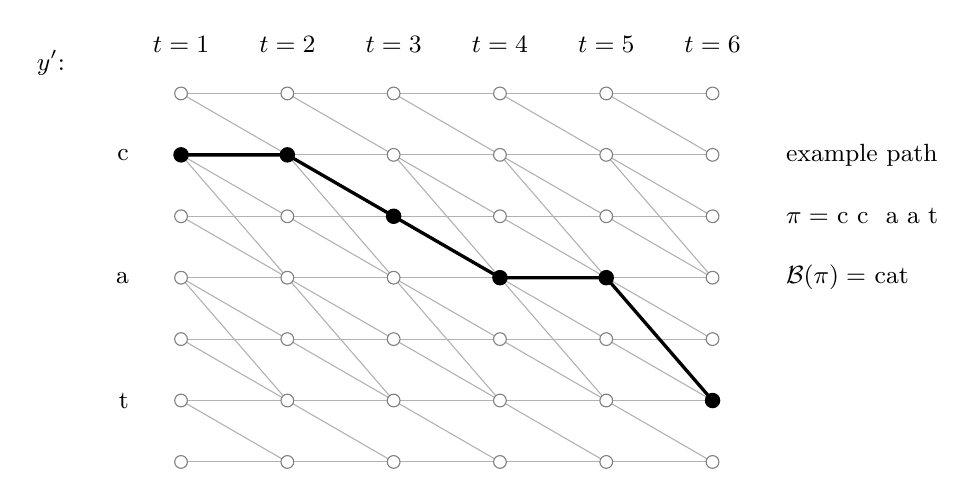
\begin{tikzpicture}[x={(1.35cm,0)},y={(0,-0.78cm)}]
\foreach \t in {1,...,5} {
  \foreach \s in {1,...,7} {\draw[gray!60] (\t,\s) -- (\t+1,\s);}
  \foreach \s in {1,...,6} {\draw[gray!60] (\t,\s) -- (\t+1,\s+1);}
  \draw[gray!60] (\t,2) -- (\t+1,4);
  \draw[gray!60] (\t,4) -- (\t+1,6);
}
\foreach \t in {1,...,6} {\foreach \s in {1,...,7} {\fill[white,draw=gray] (\t,\s) circle (2.3pt);}}
\foreach \s/\l in {1/$\varnothing$,2/c,3/$\varnothing$,4/a,5/$\varnothing$,6/t,7/$\varnothing$} {\node[font=\small,anchor=east] at (0.6,\s) {\l};}
\foreach \t in {1,...,6} {\node[font=\small,anchor=south] at (\t,0.5) {$t=\t$};}
\draw[very thick] (1,2) -- (2,2) -- (3,3) -- (4,4) -- (5,4) -- (6,6);
\foreach \t/\s in {1/2,2/2,3/3,4/4,5/4,6/6} {\fill (\t,\s) circle (2.8pt);}
\node[font=\small,anchor=west] at (6.6,2) {example path};
\node[font=\small,anchor=west] at (6.6,3) {$\pi=$ c c $\varnothing$ a a t};
\node[font=\small,anchor=west] at (6.6,4) {$\mathcal B(\pi)=$ cat};
\node[font=\small,anchor=east] at (0.0,0.5) {$y'$:};
\end{tikzpicture}
\caption{CTC lattice for the word ``cat'' with $T=6$ steps. The rows are the positions of the blank-augmented label $y'$; thin lines are the allowed transitions of Equation~\ref{eq:rec-alpha} (stay, advance, and skip over a blank between different letters). The thick path is one of the many paths that collapse to the word.}
\label{fig:rec-ctc}
\end{figure}

Three conventions of the implementation of Equations~\ref{eq:rec-ctcprob} to~\ref{eq:rec-ctcgrad} matter for the losses quoted below.
Each line's loss is divided by its target length, so every loss quoted below is a per-character negative log-likelihood, and lines with no valid path are given zero loss.
Every line of a batch uses the full $T=160$ steps including the padding.
A label cap of 120 characters, $\lfloor160\cdot0.75\rfloor$, keeps every label far below $T$, which CTC requires: it needs $T\ge U$ plus the number of adjacent repeated letters of the target.


\paragraph{Decoding.}
At inference the most probable symbol of each step is taken, repeats are merged and blanks deleted, which is the best-path (greedy) decoding of Graves \emph{et al.}~\cite{graves2006}, Equation~\ref{eq:rec-greedy}:
\begin{equation}
\hat\pi_t=\arg\max_k y_t^k,\qquad \hat y=\mathcal B(\hat\pi).
\label{eq:rec-greedy}
\end{equation}
In Equation~\ref{eq:rec-greedy}, $y_t^k$ is the probability of class $k$ at step $t$, $\hat\pi$ the path of per-step arg-maxima and $\mathcal B$ the many-to-one map defined above that merges repeats and deletes blanks.
This best-path decoding approximates $\arg\max_y p(y\mid x)$ in 160 arg-max operations; no lexicon, language model or beam search is used.
The published design reaches its best error rate with lexicon-constrained decoding, which was not implemented here, so that publication's headline figure is not a result of this project.

\subsubsection{Training data and splits}

Table~\ref{tab:rec-data} lists the data sets, the rule separating training from validation data, and the leakage each rule leaves.

\begin{table}[h]
\centering
\fontsize{9.5}{11.5}\selectfont
\begin{tabularx}{\linewidth}{|p{2.8cm}|p{3.6cm}|X|}
\hline
\textbf{Data set} & \textbf{Split rule} & \textbf{Caveat on the validation figure} \\
\hline
Lines segmented by the student's own block from scanned database pages, with labels generated by alignment (first stage only) &
The last labelled page of every writer is held out. &
Same writers in training and hold-out, so the figure is writer-dependent; the labels are project-generated and noisy. \\
\hline
Public line-level IAM transcription set: 6\,482 training, 976 validation, 2\,915 test lines (6\,481, 976 and 2\,915 after label cleaning) &
Official training, validation and test partitions. &
The validation set drives learning-rate decay and checkpoint choice, so its accuracy is mildly optimistic; the test set is used for no decision. The partitions are believed, but not verified, to be writer-independent, and the warm start from the first stage may have seen some of the same forms. \\
\hline
13 photographed pages of the two personal writers (8 and 5 pages), 355 transcription lines of which one is a diagram marker. \mustdo{This row describes the two-writer personal set. The project now has five personal writers, 30 photographed pages and 669 transcription lines, and Section~\ref{sec:results} reports the recogniser's accuracy on all 669 of them while stating that those writers appear in its fine-tuning data. Confirm which personal set the deployed recogniser was actually fine-tuned on, and correct this row and the one below to match. I could not establish this from the saved checkpoints.} &
Per page, 15\,\% of the lines (at least one) are drawn at random with a fixed seed as validation; about 52 validation lines in total. &
Validation lines come from the same pages, pen, paper, lighting and vocabulary as training lines; the figure measures ``same writer, same notebook, new lines'' and is optimistic. It also takes part in checkpoint selection. \\
\hline
Ten-author hold-out (eight database writers and two of the personal writers) &
Used only as an evaluation set. &
The held-out database lines may have been seen in the line-level training data, and their labels are project-generated, so the figure is not a writer-independent measure. \\
\hline
\end{tabularx}
\caption{Data sets of the text recogniser and their leakage assessment.}
\label{tab:rec-data}
\end{table}

In short, the first-stage hold-out is writer-dependent with noisy labels; the public set's validation split drives learning-rate decay and checkpoint choice, so its accuracy is mildly optimistic, while its test split is used for no decision, although the partitions are only believed, not verified, to be writer-independent; the personal validation lines are random lines of the same pages as the training lines (optimistic); and the ten-author hold-out may overlap the training data and has project-generated labels.
The labels of the database pages were generated by aligning the printed prompt words with the detected ink word runs by dynamic programming, the Needleman--Wunsch global alignment~\cite{needleman1970} with the project's own cost. An earlier purely proportional labelling assigned wrong text to lines; correcting the evaluation labels, with no change of the weights, raised the measured accuracy on the ten-author hold-out from 42.7\,\% to 89.4\,\%.
Label quality, not the network, had limited the earlier measurements, which is why the recogniser was later trained on a public line-level set with clean labels.

\paragraph{Data augmentation.}
Training images, and never validation images, are augmented after the resize to $64\times640$ with at most one of four geometric transformations: horizontal shear, rotation, elastic distortion~\cite{simard2003} and perspective distortion.
Each of the four is enabled independently with probability 0.5; if none is enabled the image is unchanged, otherwise one of the enabled ones is chosen uniformly, so that $P(\text{no augmentation})=1/16=6.25\,\%$ and at most one transformation acts on an image.
The transformations are a horizontal \emph{shear} with factor $k\sim U(-0.6,0.6)$ (angle $\arctan k$), a \emph{rotation} by an angle in $U(-2.5^\circ,2.5^\circ)$, an \emph{elastic distortion}~\cite{simard2003} in which random displacement fields (uniform in $[-1,1]$ per pixel) are smoothed with a Gaussian of standard deviation $\sigma\in\{3,4\}$ and scaled by $\alpha\in\{15,20\}$ before the image is warped, and a \emph{perspective} distortion in which each corner is moved by up to $d\,W/2$ horizontally and $d\,H/2$ vertically with $d\sim U(0.03,0.08)$, where $W$ and $H$ are the canvas width and height.
The fill colour of the geometric transformations is white.
No colour, contrast, noise or blur augmentation and no synthetic pre-training data are used.

\subsubsection{Training procedure}

\paragraph{Optimiser.}
The loss of Equation~\ref{eq:rec-ctcprob} is minimised by mini-batch gradient descent with the RMSprop update of Tieleman and Hinton~\cite{tieleman2012}, Equation~\ref{eq:rec-rmsprop}: for the gradient $g_t$ at update $t$, learning rate $\eta$ and weight decay $\lambda=10^{-5}$ (an L2 term added to the gradient), the update is
\begin{equation}
g_t\leftarrow g_t+\lambda\theta_{t-1},\qquad v_t=\rho\,v_{t-1}+(1-\rho)\,g_t^2,\qquad \theta_t=\theta_{t-1}-\eta\,\frac{g_t}{\sqrt{v_t}+\epsilon},
\label{eq:rec-rmsprop}
\end{equation}
with $\theta$ the parameters, $v_t$ the running average of the squared gradient (smoothing $\rho=0.99$) and $\epsilon=10^{-8}$; there is no momentum in Equation~\ref{eq:rec-rmsprop}.
Dividing the step by the square root of that running average gives every parameter its own step size, which suits the very different gradient magnitudes of convolutional and recurrent layers.
In the joint stage the global gradient norm is clipped at 5 by the rule of Pascanu \emph{et al.}~\cite{pascanu2013}, Equation~\ref{eq:rec-clip},
\begin{equation}
g\leftarrow g\,\min\Bigl(1,\frac{5}{\|g\|_2}\Bigr),
\label{eq:rec-clip}
\end{equation}
$g$ being the concatenated gradient of all parameters and $\|g\|_2$ its Euclidean norm; the clip of Equation~\ref{eq:rec-clip} stops a rare exploding gradient of the recurrent layers from destroying the weights, and batches with a non-finite loss are skipped.
A plateau schedule halves the learning rate: after a number of validation checks (the patience) without improvement of the validation loss, $\eta\leftarrow\max(0.5\,\eta,\eta_{\min})$, with $\eta$ the learning rate of Equation~\ref{eq:rec-rmsprop} and $\eta_{\min}$ a floor below which it is not reduced.
The patience of each stage, its floor $\eta_{\min}$ (which was $10^{-5}$ or $10^{-6}$) and its restart rule are listed in Table~\ref{tab:rec-stages}.

\paragraph{Staged recipe.}
Training was carried out in four stages (Table~\ref{tab:rec-stages}, Figure~\ref{fig:rec-stages}), and each stage is motivated by a limitation that was found in the previous one.
\begin{enumerate}
\item \emph{Base stage.} The published recipe was reproduced on lines that were segmented from database pages by the student's own tools. The data turned out to be small and noisy because of the labelling defect and segmentation errors, and the best validation loss was 1.06.
\item \emph{Clean-label stage.} The network was warm-started from the base stage and trained on the public line-level IAM set, whose human-checked labels remove all segmentation and labelling noise.
\item \emph{Personal fine-tuning (rejected).} Fine-tuning on the personal lines alone raised the accuracy on the personal validation lines but reduced the accuracy on the general data by about ten points (catastrophic forgetting, Table~\ref{tab:rec-forget}); freezing the convolutional layers reduced the forgetting only slightly.
\item \emph{Joint stage.} Training continues from the clean-label stage on both data sets at once, with a weighted sampler: each public line receives the weight $w_T=(1-f)/n_T$ and each personal line $w_P=f/n_P$, where $n_T=6\,481$, $n_P\approx280$ and $f=0.20$, and $n_T$ indices are drawn per epoch with replacement with probability proportional to the weights, Equation~\ref{eq:rec-sampler},
\begin{equation}
P(i)=\frac{w_i}{\sum_jw_j}.
\label{eq:rec-sampler}
\end{equation}
In expectation the sampler of Equation~\ref{eq:rec-sampler} draws 20\,\% of every epoch ($\approx1\,296$ draws) from the personal set, so that each personal line is seen about 4.6 times per epoch with fresh random augmentation, and 80\,\% from the public set. The checkpoint of the epoch with the largest $\min(\text{accuracy}_{\mathrm{public}},\text{accuracy}_{\mathrm{personal}})$ is kept, so that neither domain is sacrificed. This stage wrote the checkpoint file \texttt{paper\_cnn\_bilstm\_ctc\_joint\_best.npz}, which is the file every accuracy quoted for stage~4 was measured on.
\end{enumerate}

\begin{table}[h]
\centering
\fontsize{9.5}{11.5}\selectfont
\begin{tabularx}{\linewidth}{|l|l|l|l|l|l|X|}
\hline
\textbf{Stage} & \textbf{Data} & \textbf{$\eta_0$} & \textbf{Batch} & \textbf{Epochs} & \textbf{Clip} & \textbf{Schedule and selection} \\
\hline
Base & own lines & $10^{-3}$ & 16 & $\le200$ & none & halve after 5 stalls; stop after 15; up to 3 restarts from the best weights; best validation loss \\
\hline
Clean labels & public set & $10^{-3}$ & 16 & $\le200$ & none & as above, up to 8 restarts; best public validation loss \\
\hline
Personal & personal lines & $3\!\times\!10^{-4}$ & 8 & 60 & 5 & halve after 5 stalls; best personal validation loss \\
\hline
Joint & both, $f=0.20$ & $5\!\times\!10^{-4}$ & 16 & 30 & 5 & halve after 4 stalls on the sum of both validation losses; best $\min$ of the two accuracies \\
\hline
\end{tabularx}
\caption{Hyper-parameters of the four training stages. All stages use RMSprop~\cite{tieleman2012} (Equation~\ref{eq:rec-rmsprop}) with weight decay $10^{-5}$; the minimum learning rate was $10^{-5}$ or $10^{-6}$.}
\label{tab:rec-stages}
\end{table}

\begin{figure}[h]
\centering
\begin{tikzpicture}[x=1cm,y=1cm]
\tikzset{sb/.style={w2box,text width=3.6cm,minimum height=1.4cm}}
\node[sb] (b) at (-5.4,0) {\textbf{1 Base}\\ own database lines, noisy labels\\ best val. loss 1.06};
\node[sb] (h) at (-0.6,0) {\textbf{2 Clean labels}\\ public line set, 6\,481 lines\\ val./test 93.87/91.60\,\%};
\node[sb] (n) at (4.5,1.2) {\textbf{3 Personal only (rejected)}\\ val./test 84.26/80.56\,\%\\ personal 90.2\,\%};
\node[sb] (j) at (4.5,-1.2) {\textbf{4 Joint, 80/20 sampler}\\ val./test 94.03/91.82\,\%\\ personal 89.64\,\%};
\draw[w2arr] (b)--(h) node[midway,above,font=\scriptsize] {warm start};
\draw[w2arr] (h.east) -- ++(0.45,0) |- (n.west);
\draw[w2arr] (h.east) -- ++(0.45,0) |- (j.west);
\end{tikzpicture}
\caption{Staged training recipe of the text recogniser with the character accuracies (public validation and test sets, and personal validation; see Table~\ref{tab:rec-results} for the caveats). Stage~2 wrote \texttt{paper\_cnn\_bilstm\_ctc\_hf\_best.npz}, stage~3 \texttt{paper\_cnn\_bilstm\_ctc\_personal\_best.npz} and stage~4 \texttt{paper\_cnn\_bilstm\_ctc\_joint\_best.npz}; every accuracy in the figure was measured on the stage's own file. The checkpoint the deployed server actually loads is a different, later one, \texttt{paper\_cnn\_bilstm\_ctc\_scratch\_best.npz}, for which no accuracy is reported anywhere in this report (see below).}
\label{fig:rec-stages}
\end{figure}

Table~\ref{tab:rec-forget} sets the three ways of adding the personal data side by side.

\begin{table}[h]
\centering
\fontsize{9.5}{11.5}\selectfont
\begin{tabular}{|l|r|r|r|}
\hline
\textbf{Training} & \textbf{Public val./test (\%)} & \textbf{Personal val. (\%)} & \textbf{Remark} \\
\hline
Clean-label stage only & 93.87 / 91.60 & -- & before personal data \\
Personal only, all layers & 84.26 / 80.56 & 90.2 & forgetting \\
Personal only, frozen convolutions & 85.87 / 82.62 & 88.5 & forgetting \\
Joint, 80/20 sampler & 94.03 / 91.82 & 89.64 & both domains kept \\
\hline
\end{tabular}
\caption{The catastrophic-forgetting experiment: character accuracies of the three ways of adding personal data. Every figure in the table was measured on the stage's own checkpoint file, the last row on \texttt{paper\_cnn\_bilstm\_ctc\_joint\_best.npz}; none of them was measured on the from-scratch checkpoint that the server loads.}
\label{tab:rec-forget}
\end{table}

\paragraph{Which checkpoint is deployed.}
Four text checkpoints exist in \texttt{Software/CNN/weights}, and the quoted accuracies belong to three of them: \texttt{paper\_cnn\_bilstm\_ctc\_hf\_best.npz} from the clean-label stage (93.87\,\% public validation, 91.60\,\% public test), \texttt{paper\_cnn\_bilstm\_ctc\_personal\_best.npz} from the rejected personal-only stage (84.26/80.56\,\% public, 90.2\,\% personal) and \texttt{paper\_cnn\_bilstm\_ctc\_joint\_best.npz} from the joint stage (94.03/91.82\,\% public, 89.64\,\% personal), the figures of Table~\ref{tab:rec-forget} and Figure~\ref{fig:rec-stages}.
The fourth file, \texttt{paper\_cnn\_bilstm\_ctc\_scratch\_best.npz}, is the output of the from-scratch trainer of Section~\ref{sec:textrec-numpynn}, and it is the file the deployed system actually uses: the loader prefers it over the joint checkpoint whenever it exists, which it does, so the server serves the from-scratch weights and not the joint ones.
This matters for every accuracy in this subsection, because no accuracy of the from-scratch checkpoint is reported anywhere in this report.
Its training produced no log, and unlike the resumable runs described below its stored file contains weights and batch-normalisation statistics only, with no epoch number and no best validation score, so neither its selected epoch nor its accuracy can be recovered from the file.
The honest position is therefore that the four-stage recipe and its accuracies describe the joint checkpoint, while the deployed path loads a later checkpoint of the same architecture whose accuracy has not been measured.
\mustdo{resolve the checkpoint question before submission: either re-run the evaluation of Table~\ref{tab:rec-results} on \texttt{paper\_cnn\_bilstm\_ctc\_scratch\_best.npz} and quote its public validation, public test and personal-crop accuracies beside the joint figures, or state explicitly which single checkpoint is being submitted as the deployed recogniser and remove the other from the loader's search path so that the quoted figures and the served weights are the same file.}

A sweep over learning rate, LSTM width, depth, convolution width, dropout and optimiser (14 configurations of 50 epochs) was programmed, but no result file was kept, so the deployed architecture is the published one and not an optimum found by the student.
Training was done offline on a general-purpose computer; the training log of the joint stage was not kept, so epoch-by-epoch curves cannot be shown, and the stored joint checkpoint contains weights only.

\subsubsection{From-scratch forward-and-backward implementation}
\label{sec:textrec-numpynn}

Only work done from first principles counts for credit in this report, so a framework supplying ready-made layers and automatic differentiation would earn no credit for the recogniser's training.
The student therefore wrote one Python module that implements, from the defining equations and with no machine-learning library, the forward \emph{and} the backward (gradient) pass of every layer used by the recogniser and the two writer classifiers of Section~\ref{sec:writerid}, together with the two optimiser updates, the learning-rate schedules and the gradient-norm clip, so that no machine-learning framework supplies any layer, any gradient or any optimiser used in training.
The scope of that claim is stated precisely at the end of this subsection: it is a claim about the learning machinery, not a claim that the training programs import nothing at all.

\paragraph{Layers implemented from first principles.}
The module implements, from the defining equations and with no machine-learning library, the forward and the backward pass of the convolution of Equation~\ref{eq:rec-conv}, batch normalisation in its training form (batch statistics, Equation~\ref{eq:rec-bn}) and its folded inference form (Equation~\ref{eq:rec-bnfold}), the rectified linear unit, max-pooling and the two adaptive pools of Equations~\ref{eq:rec-hmax} and~\ref{eq:wid-pool}, a fully connected (linear) layer, dropout, the multilayer bidirectional LSTM of Equations~\ref{eq:rec-lstm} and~\ref{eq:rec-bi}, and the CTC forward--backward recursion of Equations~\ref{eq:rec-alpha} to~\ref{eq:rec-ctcgrad}.
It also implements the RMSprop update of Equation~\ref{eq:rec-rmsprop}, the AdamW update of the writer classifiers (Equations~\ref{eq:wid-adamwmom} and~\ref{eq:wid-adamw}), the plateau and cosine learning-rate schedules and the gradient-norm clip of Equation~\ref{eq:rec-clip}, so that no layer, no gradient and no optimiser update used in training comes from a machine-learning framework.
One shared training program calls it to build and train either the recogniser or a writer classifier, since the two share the convolutional backbone (Section~\ref{sec:writerid}).
The convolutional stack, the pooling layers and the fully connected layer are also called in their inference (eval) form by the validation step at the end of every epoch and by the deployed program on the single-board computer, so training, validation and deployment are three uses of one implementation.
The framework alternative would have earned no credit for the recogniser's training even though the student designed the architecture and data pipeline around it.

\paragraph{Exactly what the training code does and does not import.}
The claim made above is deliberately narrower than ``no external library at all'', because the latter would not be true, and the difference is worth stating exactly.
Every layer forward pass, every backward pass, both optimisers, both learning-rate schedules and the gradient-norm clip are in the student's own module \texttt{NumpyNN.py}, which imports nothing but \texttt{numpy}; the module contains no machine-learning import of any kind, and the from-scratch trainer builds and trains both the recogniser and the writer classifiers out of it alone.
The data pipeline that feeds that trainer does use two image-processing utilities from SciPy, and only two.
The first is \texttt{scipy.ndimage}, from which \texttt{gaussian\_filter} and \texttt{map\_coordinates} are imported at \texttt{Software/CleanPipeline/TrainText.py:27} and used to smooth the random displacement fields and to resample the warped image in the elastic distortion described above (\texttt{TrainText.py:175--180}); an equivalent separable Gaussian blur and bilinear resampling could have been written from the definitions already given in this report (Equation~\ref{eq:rec-resize} supplies the interpolation), and that they were not is a convenience and not a dependence of the learning algorithm.
The second is \texttt{scipy.signal.find\_peaks}, imported at \texttt{Software/CleanPipeline/ExtractIAMLines.py:12} and used once, to locate the minima of the smoothed row-ink profile when lines are cut out of a database page.
The from-scratch trainer \texttt{TrainScratch.py} reuses the data loaders of \texttt{TrainText.py} and \texttt{TrainAuthor.py} and therefore inherits both of these, and it also depends on the Python imaging library for reading and resizing image files.
Neither utility touches a weight, a gradient or an update: elastic distortion acts on the input image before Equation~\ref{eq:rec-norm}, and peak finding acts on a page before any line exists.
The defensible statement, and the one this report makes, is therefore that \emph{no machine-learning framework supplies any layer, gradient or optimiser}, while two SciPy image-processing utilities (Gaussian smoothing with resampling for the elastic augmentation, and peak finding for line cutting) and the imaging library are used in the data pipeline around the network.
One further library, the data-set reader used by \texttt{ExportTekliaLines.py} to export the public line images once to disk, is used outside training altogether and never during it.

\paragraph{Backward passes derived by hand.}
The forward equations of every layer have been given above; this paragraph gives the backward equations that go with them, because it is the backward passes, and not the forward ones, that a framework would otherwise have supplied, and a gradient that is merely exhibited as code has not been derived.
Throughout, $\mathcal L$ is the scalar loss and, for a tensor $A$ appearing in a forward equation, $\mathrm dA$ denotes the tensor of partial derivatives $\partial\mathcal L/\partial A$, of the same shape as $A$; $\mathrm dA$ is precisely what the module's backward function for that layer returns to its caller, $\mathrm dY$ is the gradient arriving from the layer above, $\odot$ is the element-wise product and $\mathbb 1[\cdot]$ the indicator function.
Each equation below is checked by one or more configurations of the numerical check of the next paragraph, and the correspondence between the two is stated there.

\emph{Two-dimensional convolution.} Differentiating the forward sum of Equation~\ref{eq:rec-conv} with respect to its three arguments gives
$\mathrm dW[o,c,u,v]=\sum_{n,i,j}\mathrm dY[n,o,i,j]\,X_{\mathrm{pad}}[n,c,si+u,sj+v]$ for the weights,
a plain sum over batch and position for the bias, and a sum over every window in which a given input pixel appears for the input.
Since the column of $\mathrm{cols}_n$ indexed by the output position $(i,j)$ holds exactly those entries $X_{\mathrm{pad}}[n,c,si+u,sj+v]$ for all $(c,u,v)$, the first of these is a matrix product, and the implementation evaluates the three gradients of Equation~\ref{eq:rec-im2col} as Equation~\ref{eq:rec-convbw},
\begin{equation}
\mathrm d\tilde W=\sum_{n=1}^{B}\mathrm dY_n\,\mathrm{cols}_n^{\top},\qquad
\mathrm db_o=\sum_{n,i,j}\mathrm dY[n,o,i,j],\qquad
\mathrm d\,\mathrm{cols}_n=\tilde W^{\top}\,\mathrm dY_n,
\label{eq:rec-convbw}
\end{equation}
in which the sum for $\mathrm db_o$ runs over the batch and over all $H_{\mathrm{out}}W_{\mathrm{out}}$ output positions, $B$ is the batch size, $\mathrm dY_n\in\mathbb R^{C_{\mathrm{out}}\times H_{\mathrm{out}}W_{\mathrm{out}}}$ is the incoming gradient of sample $n$ with its two spatial axes flattened, $\mathrm{cols}_n$ is that sample's im2col matrix from Equation~\ref{eq:rec-im2col}, $\tilde W\in\mathbb R^{C_{\mathrm{out}}\times C_{\mathrm{in}}k^2}$ is the reshaped weight matrix of Equation~\ref{eq:rec-im2col}, and $\mathrm d\tilde W$ is reshaped back to the four axes of $W$ before it is returned.
Both products of Equation~\ref{eq:rec-convbw} are evaluated as one batched product over $n$ (the sum over the batch being a reduction of the leading axis of the first), which is the saving quantified in Figure~\ref{fig:rec-conv2d}; the three gradients are the exact derivative of Equation~\ref{eq:rec-conv} and not an approximation of it, since Equation~\ref{eq:rec-im2col} is Equation~\ref{eq:rec-conv} rearranged.
The input gradient is then returned from the columns to the image by the col2im operation of Equation~\ref{eq:rec-col2im},
\begin{equation}
\begin{gathered}
\mathrm dX_{\mathrm{pad}}[n,c,r,q]=\sum_{u=0}^{k-1}\sum_{v=0}^{k-1}\mathrm d\,\mathrm{cols}\bigl[n,\,(c,u,v),\,(r-u,\;q-v)\bigr],\\
\mathrm dX=\mathrm dX_{\mathrm{pad}}\bigl[\,\cdot\,,\,\cdot\,,\;p{:}p{+}H,\;p{:}p{+}W\,\bigr],
\end{gathered}
\label{eq:rec-col2im}
\end{equation}
where $(r,q)$ is a position of the zero-padded input, $(c,u,v)$ indexes the rows of $\mathrm{cols}$ as channel and kernel offset, terms whose output index $(r-u,q-v)$ falls outside the $H_{\mathrm{out}}\times W_{\mathrm{out}}$ grid are zero, and the second expression of Equation~\ref{eq:rec-col2im} discards the $p$-pixel border that padding added, recovering a gradient of the same shape as the layer's input.
Equation~\ref{eq:rec-col2im} is the transpose of the im2col rearrangement and it must \emph{accumulate}: for $k>1$ the windows overlap, so one input pixel appears in up to $k^2=9$ columns and receives one contribution from each.
The implementation therefore realises it as a scatter-add, a loop of nine slice additions into a zero-initialised padded array; a reshape alone, which would be correct for non-overlapping windows, would here keep one contribution in nine and is the single most likely place for a convolution backward pass to be silently wrong.

\emph{Batch normalisation in its training form.} The learned parameters of Equation~\ref{eq:rec-bn} differentiate immediately, as Equation~\ref{eq:rec-bnbw},
\begin{equation}
\mathrm d\gamma_c=\sum_{n,i,j}\mathrm dY[n,c,i,j]\,\hat x[n,c,i,j],\qquad
\mathrm d\beta_c=\sum_{n,i,j}\mathrm dY[n,c,i,j],\qquad
\mathrm d\hat x=\gamma_c\,\mathrm dY,
\label{eq:rec-bnbw}
\end{equation}
where $\hat x$ is the normalised activation of Equation~\ref{eq:rec-bn}, $\gamma_c$ and $\beta_c$ the scale and shift of channel $c$, and every sum runs over the batch index $n$ and both spatial axes $(i,j)$ of that channel.
The input gradient is harder, because the mean $\mu_B$ and the variance $\sigma_B^2$ of Equation~\ref{eq:rec-bn} are themselves functions of every element of the channel: perturbing one element changes the output through three routes, directly through $\hat x$, through $\mu_B$ and through $\sigma_B^2$.
Collecting the three routes gives the single expression of Equation~\ref{eq:rec-bnbwx}, the form the module implements,
\begin{equation}
\mathrm dx=\frac{1}{N\sqrt{\sigma_B^2+\varepsilon}}\Bigl(N\,\mathrm d\hat x\;-\;\sum_{n,i,j}\mathrm d\hat x\;-\;\hat x\sum_{n,i,j}\bigl(\mathrm d\hat x\odot\hat x\bigr)\Bigr),
\label{eq:rec-bnbwx}
\end{equation}
in which $N=BHW$ is the number of elements of the channel over which Equation~\ref{eq:rec-bn} takes its statistics, $\varepsilon=10^{-5}$, and the two sums are scalars per channel that are broadcast back over all $N$ positions.
The three terms of Equation~\ref{eq:rec-bnbwx} are the three routes in order, and the two sums are what couples all $N$ elements of a channel: training-form batch normalisation is the one layer in this network whose backward pass cannot be written element by element, and Equation~\ref{eq:rec-bnbwx} computes all $N$ derivatives in one pass over the channel instead of $N$ separate ones.
Equation~\ref{eq:rec-bnbwx}, and not the folded inference map of Equation~\ref{eq:rec-bnfold}, is the form that is differentiated, because the folded form is never trained through: the running statistics receive no gradient at all, being updated outside the gradient path by $\mu_{\mathrm{run}}\leftarrow(1-m)\mu_{\mathrm{run}}+m\,\mu_B$ with momentum $m=0.1$, the variance by its unbiased estimate $\sigma_B^2N/(N-1)$.

\emph{Rectified linear unit and dropout.} Both are masks, and both backward passes re-apply the mask the forward pass recorded, Equation~\ref{eq:rec-relubw}:
\begin{equation}
\mathrm dx=\mathrm dY\odot\mathbb 1[x>0]\quad\text{(rectifier)},\qquad
\mathrm dx=\mathrm dY\odot M,\quad M_k=\frac{\mathbb 1[\xi_k\ge p]}{1-p}\quad\text{(dropout)},
\label{eq:rec-relubw}
\end{equation}
where $x$ is the rectifier's input, $M$ the inverted-dropout mask of Equation~\ref{eq:wid-head} with keep probability $1-p$ and $\xi_k$ the uniform draw of unit $k$.
The kink of the rectifier at $x=0$ is assigned the derivative zero in Equation~\ref{eq:rec-relubw}, which is the usual convention and is the reason the numerical check of that layer is run on inputs that keep every element away from the kink.

\emph{Max-pooling and the two adaptive pools.} A maximum is a selector, so it routes the whole incoming gradient to the element that won and nothing to the others, Equation~\ref{eq:rec-poolbw}:
\begin{equation}
\mathrm dX[n,c,2i+u,2j+v]=\begin{cases}\mathrm dY[n,c,i,j], & (u,v)=a^{\star}(n,c,i,j),\\[2pt] 0,&\text{otherwise,}\end{cases}
\label{eq:rec-poolbw}
\end{equation}
with $a^{\star}(n,c,i,j)=\arg\max_{u,v\in\{0,1\}}X[n,c,2i+u,2j+v]$ the within-window arg-max that the forward pass of the $2\times2$ pool stored in its cache, and $u,v\in\{0,1\}$ ranging over the window of output position $(i,j)$.
Because the stride equals the kernel, the windows of Equation~\ref{eq:rec-poolbw} tile the input without overlapping, so the routed values can be written into place directly and, unlike Equation~\ref{eq:rec-col2im}, no accumulation is needed.
The height maximum of Equation~\ref{eq:rec-hmax} and the width mean of Equation~\ref{eq:wid-pool} differentiate to the two halves of Equation~\ref{eq:rec-adaptbw},
\begin{equation}
\begin{gathered}
\mathrm dF[n,c,i,t]=\mathbb 1\bigl[\,i=r^{\star}(n,c,t)\,\bigr]\,\mathrm dz_t[n,c],\qquad r^{\star}(n,c,t)=\arg\max_iF[n,c,i,t],\\
\mathrm dm[n,c,t]=\frac{1}{T}\,\mathrm df[n,c],
\end{gathered}
\label{eq:rec-adaptbw}
\end{equation}
where $r^{\star}$ is the winning row cached by the forward pass of Equation~\ref{eq:rec-hmax} and $T=160$ the number of columns the mean of Equation~\ref{eq:wid-pool} runs over.
The first half of Equation~\ref{eq:rec-adaptbw} sends the gradient of a time step to the one row that supplied its value, so a feature that is never the column maximum receives nothing, which is the gradient-side price of discarding vertical position in Equation~\ref{eq:rec-hmax}.
The second half spreads the gradient of a pooled feature evenly over all 160 columns including the white padding of a short line, the exact counterpart of the dilution noted after Equation~\ref{eq:wid-pool}.

\emph{Fully connected layer.} With every axis but the last flattened into one index, Equation~\ref{eq:rec-linbw} holds:
\begin{equation}
\mathrm dW=\mathrm dY^{\top}X,\qquad \mathrm db=\sum_{m=1}^{M}\mathrm dY[m,\,\cdot\,],\qquad \mathrm dX=\mathrm dY\,W,
\label{eq:rec-linbw}
\end{equation}
where $X\in\mathbb R^{M\times I}$ is the input and $\mathrm dY\in\mathbb R^{M\times O}$ the incoming gradient with all leading axes collapsed into the index $m$, $W\in\mathbb R^{O\times I}$ is the weight matrix and $\mathrm dX$ is reshaped back to the input's own axes before it is returned.
That flattening is what lets one function serve both uses of the layer without change: for the recogniser's output layer of Equation~\ref{eq:rec-softmax}, $M=TB=160B$, so all 160 time steps of all lines of a batch contribute to one weight gradient, whereas for the writer classifier's head of Equation~\ref{eq:wid-head}, $M=B$.

\emph{Long short-term memory.} At step $t$ the hidden state is reached both from the layer above and from step $t+1$, and the memory only from step $t+1$, so the two gradients entering the cell are $\mathrm dh_t=\mathrm dY_t+\delta h_t$ and $\mathrm dc_t=\delta c_t+\mathrm dh_t\odot o_t\odot(1-\tanh^2c_t)$, where $\mathrm dY_t$ is the gradient of $h_t$ from above, $\delta h_t$ and $\delta c_t$ are the recurrent contributions produced by step $t+1$, and both recurrent terms are zero at $t=T$.
Differentiating the six lines of Equation~\ref{eq:rec-lstm} with $\sigma'=\sigma(1-\sigma)$ and $\tanh'=1-\tanh^2$ gives the four gate pre-activation gradients of Equation~\ref{eq:rec-lstmbw},
\begin{equation}
\begin{aligned}
\mathrm d\tilde o_t&=\mathrm dh_t\odot\tanh(c_t)\odot o_t\odot(1-o_t), &\qquad \mathrm d\tilde f_t&=\mathrm dc_t\odot c_{t-1}\odot f_t\odot(1-f_t),\\
\mathrm d\tilde i_t&=\mathrm dc_t\odot g_t\odot i_t\odot(1-i_t), &\qquad \mathrm d\tilde g_t&=\mathrm dc_t\odot i_t\odot(1-g_t^2),
\end{aligned}
\label{eq:rec-lstmbw}
\end{equation}
in which a tilde marks a gate's pre-activation, that is the argument of the $\sigma$ or $\tanh$ in Equation~\ref{eq:rec-lstm}, and $i_t$, $f_t$, $g_t$, $o_t$, $c_{t-1}$ and $\tanh(c_t)$ are the activations the forward pass cached at that step; each line of Equation~\ref{eq:rec-lstmbw} is the gradient of the cell output with respect to one gate multiplied by that gate's own activation derivative, so the forward cache makes the backward pass free of any re-evaluation.
The recursion that carries Equation~\ref{eq:rec-lstmbw} through time, the back-propagation through time proper, is Equation~\ref{eq:rec-lstmbptt},
\begin{equation}
\begin{aligned}
\mathrm d\tilde a_t&=\bigl[\,\mathrm d\tilde i_t;\;\mathrm d\tilde f_t;\;\mathrm d\tilde g_t;\;\mathrm d\tilde o_t\,\bigr]\in\mathbb R^{B\times4n},\\
\delta h_{t-1}&=\mathrm d\tilde a_t\,W_{hh},\qquad \delta c_{t-1}=\mathrm dc_t\odot f_t,\qquad \mathrm dx_t=\mathrm d\tilde a_t\,W_{ih},\\
\mathrm dW_{ih}&=\sum_{t=1}^{T}\mathrm d\tilde a_t^{\top}x_t,\qquad \mathrm dW_{hh}=\sum_{t=1}^{T}\mathrm d\tilde a_t^{\top}h_{t-1},\qquad \mathrm db_{ih}=\mathrm db_{hh}=\sum_{t=1}^{T}\mathbf 1^{\top}\mathrm d\tilde a_t,
\end{aligned}
\label{eq:rec-lstmbptt}
\end{equation}
with $n=256$ the hidden size, $W_{ih}\in\mathbb R^{4n\times I}$ and $W_{hh}\in\mathbb R^{4n\times n}$ the stacked gate matrices introduced after Equation~\ref{eq:rec-lstm}, $\mathrm d\tilde a_t$ the four gate gradients stacked in the same gate order, and $\mathbf 1^{\top}\mathrm d\tilde a_t$ the sum over the $B$ samples of the batch.
The loop of Equation~\ref{eq:rec-lstmbptt} runs from $t=T$ down to $t=1$, carries $\delta h_{t-1}$ and $\delta c_{t-1}$ into the previous step, accumulates the four parameter gradients over all 160 steps and emits $\mathrm dx_t$ for the layer below; the single concatenated $\mathrm d\tilde a_t$ mirrors the single concatenated forward product, so a step costs two matrix products of $4n=1024$ rows backwards against one forwards.
Both bias gradients of Equation~\ref{eq:rec-lstmbptt} are equal because both biases enter the same pre-activation sum in Equation~\ref{eq:rec-lstm}, a redundancy kept so that the checkpoint format matches the four-tensor convention of the inference code.
The term $\delta c_{t-1}=\mathrm dc_t\odot f_t$ is the reason the cell transports gradient over long distances: along the memory line drawn at the top of Figure~\ref{fig:rec-lstm} the gradient is multiplied only by the forget gate and never by a weight matrix, so it decays at a rate the network itself controls instead of at the fixed rate of a plain recurrent network, which is the vanishing-gradient property of Hochreiter and Schmidhuber~\cite{hochreiter1997} read backwards.
For the bidirectional layer of Equation~\ref{eq:rec-bi} the incoming gradient is split at the concatenation and the backward direction is handled by time reversal, Equation~\ref{eq:rec-lstmrev},
\begin{equation}
\mathrm d\overrightarrow h_t=\mathrm dh_t[1{:}n],\quad
\mathrm d\overleftarrow h_t=\mathrm dh_t[n{+}1{:}2n],\quad
\mathrm dx=\mathrm dx^{\rightarrow}+\mathcal R\bigl(\mathrm dx^{\leftarrow}\bigr),
\label{eq:rec-lstmrev}
\end{equation}
where $\mathcal R$ is the time-reversal operator, $(\mathcal Ru)_t=u_{T+1-t}$, and $\mathrm dx^{\rightarrow}$, $\mathrm dx^{\leftarrow}$ are the input gradients that Equation~\ref{eq:rec-lstmbptt} returns for the two directions.
The backward direction's forward pass ran on $\mathcal R(x)$, so its recursion must be driven by $\mathcal R(\mathrm d\overleftarrow h)$ and not by $\mathrm d\overleftarrow h$, and the $\mathrm dx$ it returns is in reversed time and must be reversed back, which is the second $\mathcal R$ of Equation~\ref{eq:rec-lstmrev}; omitting either reversal yields a gradient that is wrong only in its time ordering, an error the numerical check below detects at once but a falling loss curve would hide.
The two input gradients add in Equation~\ref{eq:rec-lstmrev} because both directions read the same input sequence, and for the stack of two bidirectional layers Equation~\ref{eq:rec-lstmrev} is applied to the layers in reverse order, the $\mathrm dx$ of the upper layer being the $\mathrm dY$ of the lower.

\emph{Loss layers and the complete chain.} The recogniser's loss gradient is Equation~\ref{eq:rec-ctcocc}, computed from the forward and backward recursions of Equations~\ref{eq:rec-alpha} and~\ref{eq:rec-beta} in the logarithmic domain of Equation~\ref{eq:rec-lse}; the writer classifiers' loss gradient is the cross-entropy gradient of Equation~\ref{eq:wid-cebw}.
Both are taken with respect to the pre-softmax scores, so neither the log-softmax of Equation~\ref{eq:rec-softmax} nor the softmax of Equation~\ref{eq:wid-ce} needs a backward pass of its own.
The complete backward chain of the recogniser is therefore Equation~\ref{eq:rec-ctcocc}, then Equation~\ref{eq:rec-linbw} for the output layer, then Equations~\ref{eq:rec-lstmrev} and~\ref{eq:rec-lstmbptt} once for each of the two bidirectional layers, then Equation~\ref{eq:rec-adaptbw} for the height collapse, and then, for each of the twelve convolutional units in reverse order, Equations~\ref{eq:rec-relubw}, \ref{eq:rec-bnbwx} and~\ref{eq:rec-convbw} with~\ref{eq:rec-col2im}, interrupted by Equation~\ref{eq:rec-poolbw} at the two max-pools; the writer classifiers' chain is Equation~\ref{eq:wid-cebw}, Equation~\ref{eq:rec-linbw} twice with Equation~\ref{eq:rec-relubw} between them, Equation~\ref{eq:rec-adaptbw} for both pools, and the same convolutional sequence.
The resulting gradients are then clipped by Equation~\ref{eq:rec-clip} and consumed by the updates of Equations~\ref{eq:rec-rmsprop}, \ref{eq:wid-adamwmom} and~\ref{eq:wid-adamw}.
Nothing in that chain is approximate: every equation of this paragraph is an exact derivative of a forward equation given earlier in this subsection, which is what makes the next paragraph a check of the algebra rather than a measurement of an error.

\paragraph{Verification by numerical differentiation.}
No automatic differentiation tool checks these hand-derived backward passes, so each was verified independently against the central-difference estimate of Equation~\ref{eq:rec-gradcheck},
\begin{equation}
\frac{\partial\mathcal L}{\partial\theta_i}\approx\frac{\mathcal L(\theta+\varepsilon e_i)-\mathcal L(\theta-\varepsilon e_i)}{2\varepsilon},\qquad\varepsilon=10^{-5},
\label{eq:rec-gradcheck}
\end{equation}
where, in Equation~\ref{eq:rec-gradcheck}, $e_i$ is the unit vector of parameter $i$ and $\mathcal L$ a scalar loss on a small random input.
A configuration is one (layer variant, tensor) pair; both the input gradient and the gradient with respect to every learnable parameter of that layer are checked, so one layer gives several configurations.
The 78 configurations exist for exactly one purpose, which is to test the equations of the previous paragraph, and they map onto them one for one: the three gradients of Equation~\ref{eq:rec-convbw} and the scatter-add of Equation~\ref{eq:rec-col2im} are three configurations of the convolution (one for $\mathrm d\tilde W$, one for $\mathrm db_o$ and one for the input gradient that Equation~\ref{eq:rec-col2im} assembles), repeated over the kernel, padding and channel variants the network uses; the two parameter gradients of Equation~\ref{eq:rec-bnbw} and the input gradient of Equation~\ref{eq:rec-bnbwx} are three more; the masks of Equation~\ref{eq:rec-relubw}, the routing of Equation~\ref{eq:rec-poolbw} and the two halves of Equation~\ref{eq:rec-adaptbw} are one configuration each; the three gradients of Equation~\ref{eq:rec-linbw} are three; the LSTM contributes the four parameter tensors and the input gradient of Equation~\ref{eq:rec-lstmbptt} for each direction of each layer, together with the split and the two reversals of Equation~\ref{eq:rec-lstmrev}; and the loss layers contribute the logit gradients of Equations~\ref{eq:rec-ctcocc} and~\ref{eq:wid-cebw}.
The derivations and the check are therefore one argument and not two: each equation above is a claim about a derivative, and each configuration below is the independent test of one such claim, so a passing configuration is evidence for a specific line of algebra rather than for the module in general.
A configuration is accepted when the relative difference of Equation~\ref{eq:rec-gradtol} stays below the tolerance $10^{-6}$,
\begin{equation}
\frac{\max_i\lvert g_i^{\mathrm{a}}-g_i^{\mathrm{n}}\rvert}{\max\bigl(1,\ \max_i\lvert g_i^{\mathrm{a}}\rvert+\max_i\lvert g_i^{\mathrm{n}}\rvert\bigr)}<10^{-6},
\label{eq:rec-gradtol}
\end{equation}
with $g^{\mathrm{a}}$ the analytic and $g^{\mathrm{n}}$ the numerical gradient of Equation~\ref{eq:rec-gradtol}.
Of the 78 configurations, 77 passed. The relative differences of Equation~\ref{eq:rec-gradtol} lie between $4.9\times10^{-12}$ and $1.4\times10^{-10}$, four to six orders of magnitude inside the tolerance, the agreement expected of a correct derivative at this step size.
The scalar loss used in Equation~\ref{eq:rec-gradcheck} is $\mathcal L=\sum_j o_jR_j$ for a fixed random $R$, so $\partial\mathcal L/\partial o=R$ exactly and no second approximation enters the comparison.
The check is a standalone program, \texttt{GradCheckNumpyNN.py}, part of the code submission; its full output is saved beside it.
All arithmetic is in double precision, $\varepsilon=10^{-5}$, and up to 40 randomly chosen elements of each tensor are probed (2044 elements in total).
On the stricter per-element measure $\lvert g^{\mathrm a}-g^{\mathrm n}\rvert/(\lvert g^{\mathrm a}\rvert+\lvert g^{\mathrm n}\rvert)$ the worst case over all 2044 elements is $2.0\times10^{-7}$, on a recurrent weight of the two-layer bidirectional LSTM whose gradient is itself near zero, where the central difference has no significant digits left.
Max-pooling and the rectified linear unit were checked with inputs from a permuted linear spacing, so no element lies within $\varepsilon$ of the kink of Equation~\ref{eq:rec-relubw} and no perturbation can change the arg-max $a^{\star}$ of Equation~\ref{eq:rec-poolbw}, which would otherwise make the numerical estimate compare two different selectors rather than one derivative; dropout was checked with the mask $M$ of Equation~\ref{eq:rec-relubw} held fixed, since a resampled mask changes the function between the two evaluations of Equation~\ref{eq:rec-gradcheck}; and batch normalisation was checked in its training form, Equation~\ref{eq:rec-bnbwx}, the form whose backward pass is used, so the all-to-all coupling of that equation is inside what was verified and the folded map of Equation~\ref{eq:rec-bnfold} is not relied upon.
The agreement of Equation~\ref{eq:rec-gradtol} at $4.9\times10^{-12}$ to $1.4\times10^{-10}$ is therefore the strongest single piece of evidence in this subsection that the derivations of Equations~\ref{eq:rec-convbw} to~\ref{eq:rec-lstmrev}, and the loss gradients of Equations~\ref{eq:rec-ctcocc} and~\ref{eq:wid-cebw}, are the correct derivatives of the forward equations they were derived from.

The one configuration that failed is a genuine defect, reported here rather than removed.
The CTC loss does not survive an empty label sequence: for a transcription of length $L=0$ the blank-interleaved target has $S=2L+1=1$ entry, but two of the shifted arrays that carry the recursion are built with two entries regardless of $S$, so the recursion writes a two-element array into a one-element row and raises a shape error instead of returning the loss.
Those shifted arrays are the implementation of the $s-1$ and $s-2$ terms of Equation~\ref{eq:rec-alpha} and the $s+1$ and $s+2$ terms of Equation~\ref{eq:rec-beta}, which is why the fault is confined to the lattice indexing and touches neither the transition rule nor the gradient of Equation~\ref{eq:rec-ctcocc}.
A single-character target ($S=3$) and a target with a repeated character, the case that exercises the forbidden skip transition, both pass, so this is an edge-case indexing fault and not a wrong derivative.
Its practical effect is small, because a line with no transcription never reaches the trainer, but the function is not safe against one and the fault is listed in Section~\ref{sec:discussion}.
The check also confirmed that when no alignment exists, that is when $2L+1>T$, the loss is returned as infinite with undefined gradients; this is correct for an impossible alignment, but such samples must be removed before training rather than relied upon to contribute nothing.

The gradient check runs against the batched form of each layer that the trainer uses, so the faster form is the one verified.
Every layer of the module was first written as an explicit loop over the batch, for clarity and correctness, and the batch loop was then replaced, where it dominated the running time, by one batched matrix product; Figure~\ref{fig:rec-conv2d} gives the forward and the backward code of the convolution in that batched form.

\begin{figure}[h]
\centering
\fontsize{8.5}{10}\selectfont
\begin{verbatim}
def Conv2dForward(x, w, b, padding=1):
    cols = Im2Col(x, kernelSize=3, padding=padding)      # (B, Cin*9, H*W)
    wFlat = w.reshape(w.shape[0], -1)                    # (Cout, Cin*9)
    out = (wFlat @ cols).reshape(B, Cout, H, W) + b[:, None, None]
    return out, (x, w, cols)                             # cache for backward

def Conv2dBackward(dOut, cache):
    x, w, cols = cache
    dOutFlat = dOut.reshape(B, Cout, -1)
    dw = (dOutFlat @ cols.transpose(0, 2, 1)).sum(axis=0).reshape(w.shape)
    db = dOut.sum(axis=(0, 2, 3))
    dCols = w.reshape(Cout, -1).T @ dOutFlat
    dx = Col2Im(dCols, x.shape, kernelSize=3, padding=padding)
    return dx, dw, db
\end{verbatim}
\caption{Forward and backward pass of the two-dimensional convolution, simplified from the student's implementation. The code is the implementation of the equations and not a substitute for them: \texttt{out} is Equation~\ref{eq:rec-im2col}, \texttt{dw}, \texttt{db} and \texttt{dCols} are the three gradients of Equation~\ref{eq:rec-convbw}, and \texttt{Col2Im} is the scatter-add of Equation~\ref{eq:rec-col2im}. The batch dimension $B$ is handled by a single broadcasted matrix product (\texttt{@}) rather than a Python loop over samples, which was measured to be about 35\,\% faster than an equivalent per-sample loop for a realistic training batch.}
\label{fig:rec-conv2d}
\end{figure}

\paragraph{Training speed and warm-starting.}
With no graphics processor and no vectorised automatic-differentiation engine behind it, one training step of a batch of 16 real lines took on the order of tens of seconds on a general-purpose laptop processor, substantially slower than the published-framework implementation used for the four-stage recipe above, and timing showed that an un-vectorised convolution, not the recurrent layers or the CTC loss, was the dominant cost, hence the batched matrix product of Figure~\ref{fig:rec-conv2d}.
Training is therefore not run to convergence from a random initial condition at this speed.
Instead the training program can load every tensor of an existing checkpoint whose shape matches (a warm start), so a further run only continues improving an already-competent network.
It also writes the current epoch number and the best validation score into the checkpoint after every epoch, so a run interrupted by a crash or a time limit resumes from the last completed epoch.
Complete code for this module, the shared training program and the deployed inference program has been submitted separately on the AMS.

\paragraph{Evaluation metrics.}
Accuracy is measured with the Levenshtein edit distance~\cite{levenshtein1966}, the minimum number of insertions, deletions and substitutions that turn string $a$ into string $b$, computed by the dynamic programme of Wagner and Fischer~\cite{wagner1974}, Equation~\ref{eq:rec-lev},
\begin{equation}
\begin{gathered}D[i][j]=\min\bigl(D[i-1][j]+1,\;D[i][j-1]+1,\;D[i-1][j-1]+\mathbb 1[a_i\ne b_j]\bigr),\\ D[i][0]=i,\ D[0][j]=j,\end{gathered}
\label{eq:rec-lev}
\end{equation}
with $d_{\mathrm{lev}}(a,b)=D[|a|][|b|]$ the value of Equation~\ref{eq:rec-lev} at the two full string lengths.
For training and validation the character error rate is micro-averaged over all lines $n$ with prediction $\hat y_n$ and reference $y_n$, Equation~\ref{eq:rec-cer},
\begin{equation}
\mathrm{CER}=\frac{\sum_nd_{\mathrm{lev}}(\hat y_n,y_n)}{\sum_n|y_n|},\qquad\text{character accuracy}=1-\mathrm{CER},
\label{eq:rec-cer}
\end{equation}
where $d_{\mathrm{lev}}$ is the Levenshtein edit distance; the character error rate of Equation~\ref{eq:rec-cer} is the total edit distance divided by the total reference length, the character accuracy is one minus it, and the measure is case-sensitive.
The end-to-end evaluation of Section~\ref{sec:results} instead averages per line the floored accuracy $\max(0,1-d_{\mathrm{lev}}/|y|)$ after lower-casing, which is slightly more lenient, so the two kinds of figure are not computed identically.
The word measure is implemented as the longest-common-subsequence (LCS) recall of Equation~\ref{eq:rec-wacc},
\begin{equation}
\mathrm{WordAcc}=\frac{\mathrm{LCS}(\text{reference words},\text{predicted words})}{\#\text{reference words}},
\label{eq:rec-wacc}
\end{equation}
so that Equation~\ref{eq:rec-wacc} is an in-order recall and not $1-\mathrm{WER}$; a standard word error rate $\mathrm{WER}=d_{\mathrm{lev}}(\text{word sequences})/\#\text{reference words}$ was computed only once, when the public sets were re-evaluated.

Table~\ref{tab:rec-results} sets out the measurements taken while this block was designed and the limits of what they support.
They are \emph{not} the final qualification results, which belong to Section~\ref{sec:results}, and every figure carries the caveat of its data set (Table~\ref{tab:rec-data}).

\begin{table}[h]
\centering
\fontsize{9.5}{11.5}\selectfont
\begin{tabularx}{\linewidth}{|p{3.7cm}|p{2.7cm}|X|}
\hline
\textbf{Data set} & \textbf{Result} & \textbf{Status of the figure} \\
\hline
Public set, validation (976 lines) & 94.03\,\% character accuracy; WER 21.1\,\% & Used for model selection, therefore mildly optimistic. \\
\hline
Public set, test (2\,915 lines) & 91.82\,\% character accuracy; WER 26.7\%; 15.9\,\% of lines exactly right & Used for no decision; the cleanest figure for the general benchmark, with the partition caveats of Table~\ref{tab:rec-data}. \\
\hline
\textbf{Personal crops, 669 correctly cut lines (current 13-writer system)} & \textbf{98.61\,\% character, 94.21\,\% word} & Measured on crops the segmenter produced and that were confirmed to match the label count, so segmentation failures are excluded; the writers also appear in the fine-tuning data. This is the operating figure of Section~\ref{sec:results}, not an end-to-end page figure. \\
\hline
Personal crops, per writer & Owen 99.15\,\%, Dylan 99.03\,\%, Abhinav 98.94\,\%, Yeukita 98.30\,\%, Thiya 96.46\,\% character accuracy & 75 to 206 crops each; Thiya is the weakest hand for recognition. \\
\hline
Ten personal photographed pages, full page pipeline including segmentation and label alignment & 61.21\,\% (CER 38.79\,\%, 3\,617 of 9\,324 characters) & Six unique pages (four listed twice); measured with an earlier recogniser, before the personal pages were used for fine-tuning. It is the only figure in the project that exercises the complete page-to-text chain. \\
\hline
Recognition speed, 669 crops & 8.86\,ms per character, 353\,ms per line & Against the 25\,ms per character of R4 this is a margin of about 2.8 times, on the development laptop. \\
\hline
\end{tabularx}
\caption{Accuracy of the text recogniser. The public-set figures and the full-page figure predate the final training and are retained because they are the only ones measured on an independent partition or through the complete chain; the 669-crop figure is the current operating point. The two public-set rows were measured on \texttt{paper\_cnn\_bilstm\_ctc\_joint\_best.npz}; no row of this table was measured on \texttt{paper\_cnn\_bilstm\_ctc\_scratch\_best.npz}, the checkpoint the deployed loader prefers (see ``Which checkpoint is deployed'' above).}
\label{tab:rec-results}
\end{table}

Three conclusions follow.
First, joint training kept the general accuracy while adding the personal writers (the test accuracy rose by 0.22 points over the stage with clean labels only), so the weighted sampler is justified; fine-tuning on the personal lines alone was rejected because the general accuracy fell by about ten points.
Second, the word error rate is about four times the character error rate, so roughly one word in four contains a character error and only about one line in six is entirely correct; greedy decoding without a lexicon leaves spelling errors uncorrected.
Third, the gap between the operating figure of 98.61\,\% on correctly cut crops and the 61.21\,\% through the complete page pipeline is the largest discrepancy in this report, and it shows where the remaining end-to-end loss most probably lies.
That comparison is not clean.
The two figures used different recogniser versions and different page sets, and the pages used for the full-page measurement were later included in the fine-tuning data, so an unknown part of the 37-point difference is recognition improvement rather than segmentation or label-alignment error.
What can be stated is that the crops in the operating figure were hand-checked to be correct whereas the full-page path has no such guarantee, so the difference bounds the combined effect of segmentation and label alignment from above and cannot be attributed to recognition, measured at 98.61\,\% given correct crops.
Splitting the two causes requires re-running the full page pipeline with the current recogniser on pages never used for training, the protocol proposed in Section~\ref{sec:discussion}.

\subsubsection{Inference implementation for the single-board computer}

The single-board computer runs the eval-mode form of the same module (Section~\ref{sec:textrec-numpynn}), in Python, using only array arithmetic, so no re-implementation was needed between training and deployment.
Each convolution becomes the one matrix product of Equation~\ref{eq:rec-im2col}: that optimised product replaces the six nested loops of Equation~\ref{eq:rec-conv} and was about ten times faster than a general summation routine, at the cost of memory.
Batch normalisation uses the folded form of Equation~\ref{eq:rec-bnfold}, pooling uses windowed views of the array, the height collapse is a maximum over one axis, and the LSTM is an explicit loop over the 160 steps with one product of 1024 rows per step and direction, the backward direction being a pass over the reversed sequence; the weights are read directly from the plain array checkpoint written by training, with no parsing of any third-party model format.
Before the eval-mode form was trusted, its forward pass was cross-checked, independently of the gradient check, against the training-mode forward pass on the same weights with the batch-normalisation statistics frozen: over 1358 real lines the top-1 agreement was 100.00\,\% with a maximum absolute logit difference of $7.6\times10^{-6}$.
Recognition measured 8.86\,ms per character and 353\,ms per line over 669 real crops, inside the 25\,ms per character of requirement R4 by a margin of about 2.8 times, with the model already resident in memory on the development laptop.
The earlier figure of 65 to 75\,ms per character differs by measurement conditions, not by a change of model: it was one isolated forward pass including image preparation, whereas the current figure is total inference time divided by total characters over a full run.
Timing on the ODROID N2+ was not measured, and the ARM processor is expected to be slower than the development laptop, so the margin is expected to shrink on the target hardware.
\mustdo{measure the recognition time per line on the ODROID N2+; the project files contain no such measurement, and the proposal's budget may refer to the whole classification step.}

\paragraph{The earlier separate inference implementation and its weight reader.}
Training needs a large software environment, which should not be installed on the single-board computer.
Before the single shared module above was adopted, the student therefore wrote a separate, from-scratch inference implementation in Python that reads the trained weights directly and uses only array arithmetic; it consists of three small modules (about 480 lines in total): the layer functions, the network, and a weight reader.
The training-time weight file of that design is an archive that contains a serialised object structure, in which every tensor is replaced by a reference to a storage key, and one raw little-endian byte file per storage.
The student's weight reader opens the archive, parses the object structure with a customised reader that intercepts the tensor and storage constructors, reads the bytes of each storage into an array, rebuilds every tensor from its shape and strides, and returns a dictionary of 102 arrays with the names of the training model.
The inference code then indexes the weights by name, and no machine-learning software is needed at run time.
For one random $64\times640$ input, the largest difference between the $160\times75$ log-probability matrices of that inference code and the training code was $2.3\times10^{-5}$ for the deployed weights, $1.1\times10^{-5}$ for the clean-label stage and $9.5\times10^{-6}$ for the personal stage, with identical arg-max (and therefore decoded text) at all 160 steps; this is a single synthetic input and not a test-set sweep, which is why the 1358-line comparison above was made afterwards.
The weights occupy 13.4\,MB.
On the development computer (processor only) one forward pass of one line took 2.6 to 3.1\,s; for a line of 40 characters this is about 65 to 75\,ms per character, which exceeds the 25\,ms per character that requirement R4 allows, and the ARM processor of the single-board computer is expected to be slower still.
Optional compiled replacements for the convolution and the LSTM exist but are not used: the compiled convolution was slower than the optimised matrix product on a desktop processor, and the compiled LSTM was 2.8 to 4.4 times faster than the array version.

\subsubsection{Design alternatives and justification}

Table~\ref{tab:rec-alt} compares the design with the alternatives that were considered.
Only the chosen design was built and measured; the statements about the others are arguments, not measurements.

\begin{table}[h]
\centering
\fontsize{9.5}{11.5}\selectfont
\begin{tabularx}{\linewidth}{|p{3.2cm}|X|X|}
\hline
\textbf{Alternative} & \textbf{For} & \textbf{Against} \\
\hline
Character segmentation and a per-character classifier (small convolutional network) &
Simple network; the proposal's plan. &
Needs a segmenter that works on joined letters; classification errors cannot be repaired by context; needs character-level labels that the available data lack. \\
\hline
Line-level CNN-BiLSTM-CTC (chosen) &
No segmentation below the line; alignment-free training from line transcriptions; context from both sides; output is a string; 3.36 million parameters can be run by a from-scratch implementation. &
Needs line segmentation; greedy decoding leaves spelling errors; CTC assumes independent steps. \\
\hline
Lexicon or language-model decoding &
Repairs near-miss words; gives the lowest error in the published design. &
Needs a corpus and a decoder; the technical vocabulary and symbols of the pages are largely out of vocabulary. Future work. \\
\hline
Deeper backbones with skip connections &
Easier training of very deep networks. &
The 12-layer network with batch normalisation trained well; larger models cost memory and time on the single-board computer. \\
\hline
Attention-based encoder--decoder or transformer &
Strong accuracy on large corpora. &
Far more parameters, large pre-training data, slow autoregressive decoding that can skip or invent text, and hard to implement from scratch for the board. \\
\hline
Word-level recognition &
Uses the lexicon directly. &
Needs word segmentation and a closed vocabulary; poor for names, numbers and symbols. \\
\hline
\end{tabularx}
\caption{Alternatives to the line-level recogniser.}
\label{tab:rec-alt}
\end{table}


The chosen design fits the four facts of the problem: the output is a sequence of unknown length (CTC), cursive strokes need context from both sides (bidirectional recurrence), the available labels are line transcriptions (an alignment-free loss), and the model is small enough to re-implement with matrix products and element-wise gate equations on the single-board computer.
The same convolutional backbone is reused for the writer classifiers of Section~\ref{sec:writerid} and the forced alignment of Section~\ref{sec:styleprofile}, which saves design and training effort.
